% Autor: Tony Pham xphamt00@stud.fit.vutbr.cz

\documentclass[12pt, letterpaper]{article}

\usepackage{pdfpages}
\usepackage{rotating}
\usepackage[czech]{babel}
\usepackage[utf8]{inputenc}
\usepackage[a4paper, total={6in, 8in}]{geometry}
\usepackage{graphicx} 

\begin{document}

	%%%%%%%%%%%%%%%%%%%%%%%%%%%%% Titulní stránka %%%%%%%%%%%%%%%%%%%%%%%%%%%%%%%%
	\begin{titlepage}
		\begin{center}
			\includegraphics[width=0.80\linewidth]{logo_cz.png} \\

			\vspace{\stretch{0.320}}

			\Huge{Projektová dokumentace} \\
			\LARGE{\textbf{Implementace překladače jazyka IFJ21}} \\
			\Large{Tým 047, Varianta I}
			\vspace{\stretch{0.600}}
		

			\Large
			\begin{tabular}{l l l}
			    Členové týmu: \\\\
				\textbf{Tomáš Bártů} & \textbf{(xbartu11)} & \quad 25\,\% \\
				Šimon Vacek  & (xjanec30) & \quad 25\,\% \\
				Vít Janeček  & (xjanec30) & \quad 25\,\% \\
				Tony Pham  & (xphamt00) & \quad 25\,\% \\\\\\
			\end{tabular}
		\end{center}
			{\Large \today}
		\hfill
	\end{titlepage}

	%%%%%%%%%%%%%%%%%%%%%%%%%%%%%%%% Obsah %%%%%%%%%%%%%%%%%%%%%%%%%%%%%%%%
	\pagenumbering{arabic}
	\setcounter{page}{1}
	\tableofcontents
	\clearpage
	
	%%%%%%%%%%%%%%%%%%%%%%%%%%%%% Řešení projektu %%%%%%%%%%%%%%%%%%%%%%%%%%%%%%%%
	\section{Řešení projektu}
	
	\subsection{Lexikální analýza}
    \large
	Při implementaci překladače jsme začali prvně s tvorbou lexikální analýzy.
    Hlavní funkce je \textbf{\textit{get\_token}}, která je implementována jako konečný automat a žádá 2 parametry: strukturu token (po průchodu funkcí uloží do struktury \textbf{\textit{ID}} [typy tokenů: řetězec, klíčové slovo, číslo, EOL, EOF …] a \textbf{\textit{VALUE}} [value se dále rozděluje na: string, integer, keyword, double]) a vstupní soubor. Funkce čte soubor znak po znaku a rozhoduje do jakého stavu má jít pomocí využití switche a casu pro každý stav, kde je potřeba.\\\\

	\subsection{Syntaktická analýza}
    \large
    Syntaktickou analýzu jsme implementovali rekurzivně a nachází se v \textbf{\textit{parser.c}} (top-down) a \textbf{\textit{expression.c}} (bottom-up) Vstupem jsou jednotlivé tokeny z lexikální analýzy.
    Syntaktická analyzátor využívá LL-Gramatiku (LL-Tabulku a LL-Pravidla) k tomu, aby zjistil, zda jde vstup programu syntakticky správně.\\\\
    
    \textbf{\textit{Symtable.c}} je implementovaná pomocí binárního stromu, zásobníku a jednosměrně vázaných seznamů. Základem je sktruktura \textbf{\textit{SLList\_Frame}} , která tvoří počátek vázaného seznamu. Tato struktura dále obsahuje další 2 vázané seznamy: \textbf{\textit{topLocalElement}} a \textbf{\textit{globalElement}}.\\\\
    \textbf{\textit{GlobalElement}} ukazuje na globální rámce (funkce) a tento rámec je struktura obsahující: \textbf{\textit{node}} a \textbf{\textit{previousElement}}.\\\\\\
    \textbf{\textit{TopLocalElement}} ukazuje na lokální rámce(tělo funkce, cyklus, while) a tento rámec je struktura obsahující: \textbf{\textit{node}} a \textbf{\textit{previouElement}}.\\\\
     \textbf{\textit{Node}} je ukazatel na kořen binárního stromu, kde jeho jednotlivé noty jsou struktury, které obsahují další vázané seznamy s informacemi o rámcích. \\\\
     Pro zjednodušení jsme se rozhodli neimplementovat vícenásobné přiřazení hodnot do proměnných. Rovněž neimplementujeme funkce s více návratovými hodnotami. \\
     Kvůli nejasnostem v zadaní jsme nil nebrali jako datový typ a pouze jako hodnotu. Deklarované proměnné je implicitně nastavena hodnota nil a nedá se použít, dokud není inicializována.
    
	\subsection{Sémantická analýza}
    Sématická analýza stejně jako syntaktická analýza je implementována v \textbf{\textit{parser.c}} a \textbf{\textit{expression.c}}. Při implementaci bylo nutné rozdělit jeden z neterminálu na 2 funkce které dělají různé sémantické kontroly, ale syntaxi kontrolují stejně.
	\subsection{Generování cílového kódu}
    Generování kódu pro vestavěné funkce (reads, readi, readn, write, tointeger, substr, ord, chr) je v \textbf{\textit{buildIn.c}} . Dále jsme vytvořili pomocné funkce pro generování kódu, který se často opakuje a nachází se ve \textbf{\textit{generate\_code.c}}.\\\\
    Samotné generování ifjcode21 je umístěné v \textbf{\textit{parser.c}} a \textbf{\textit{expression.c}}. Zde se generuje hlavička souboru, funkce programu, logika if a while atd. . Za zmínku stojí řešení stínění, které jsme vyřešili tak, že připisujeme proměnné ze spodku zásobníku rámců do rámce nad ním až na top.
	%%%%%%%%%%%%%%%%%%%%%%%%%%%%%%%% Práce v týmu %%%%%%%%%%%%%%%%%%%%%%%%%%%%%%%%
	\section{Práce v~týmu}

	\subsection{Způsob práce v~týmu}
    
    \large
    Na projektu jsme začali pracovat v půlce října. Ze začátku jsme si rozdělili základní úkoly a po dokončení jsme se vždy domluvili co má daný jedinec dělat dál.
    
	\subsection{Verzovací systém}
    
    \large
    Pro správu našich souborů jsme zvolili verzovací systém Git. Ten nám umožnil zpracovávat více souborů zároveň.
    
	\subsection{Komunikace}
	\large
	Jako komunikační prostředky jsme zvolili discord a massanger, kde jsme konzultovali aktuální témata k projektu. Později jsme se začali scházet ve školních prostorech, aby jsme mohli aktivněji řešit aktuální problémy. 

	\subsection{Rozdělení práce mezi členy týmu}
	\Large 
	\textbf{Tomáš Bártů:}\\
	Návrh automatu, Korekce, Syntaktická analýza zdola nahoru, Sématická analýza, Abstraktí datové struktury, Debug, Generování kódu \\

	Šimon Vacek:\\
	Testy, LL gramatika, Syntaktická analýza shora dolu, Sématická analýza, Debug, Generování kódu\\
	\\\\
	Vít Janeček:\\
	Lex. analýza, Abstraktí datové struktury včetně tabulky symbolů, Debug, Generování kódu\\
	
	Tony Pham:\\
	Lex. analýza, Dokumentace, Oprava leaků, Debug, Generování kódu\\
	
	%%%%%%%%%%%%%%%%%%%%%%%%%%%%%%% Problémy při vývoji %%%%%%%%%%%%%%%%%%%%%%%%%%
	\section{Problémy při vývoji}
	\large
    Během implementace scanneru jsme v syntaktické analýze museli řešit hned několik problému např.: přeskočení čtení znaku u některých stavů (pomohla nám funkce \textbf{\textit{ungetc}}), chybný návrh automatu (museli jsme často přidávat / opravovat stavy).
	\\
	\\
	Během syntaktické analýzy shora dolů se také projevila naše chabé dovednosti plánování. Pravidla LL gramatiky byly upraveny téměř jedenáctkrát a to i 3 dny před odevzdáním.
	\\
	\\
	Podcenili jsme časovou náročnost projektu, sice jsme začali poněkud brzy a ze začátku šlo vše bez problému, ale při implementaci Syntaktické analýzy se vývoj projektu velmi zpomalil.
	%%%%%%%%%%%%%%%%%%%%%%%%%%%% Diagram automatu %%%%%%%%%%%%%%%%%%%%%%%%%%%%%%%%
	\begin{sidewaysfigure}
        \section{Diagram automatu}
	        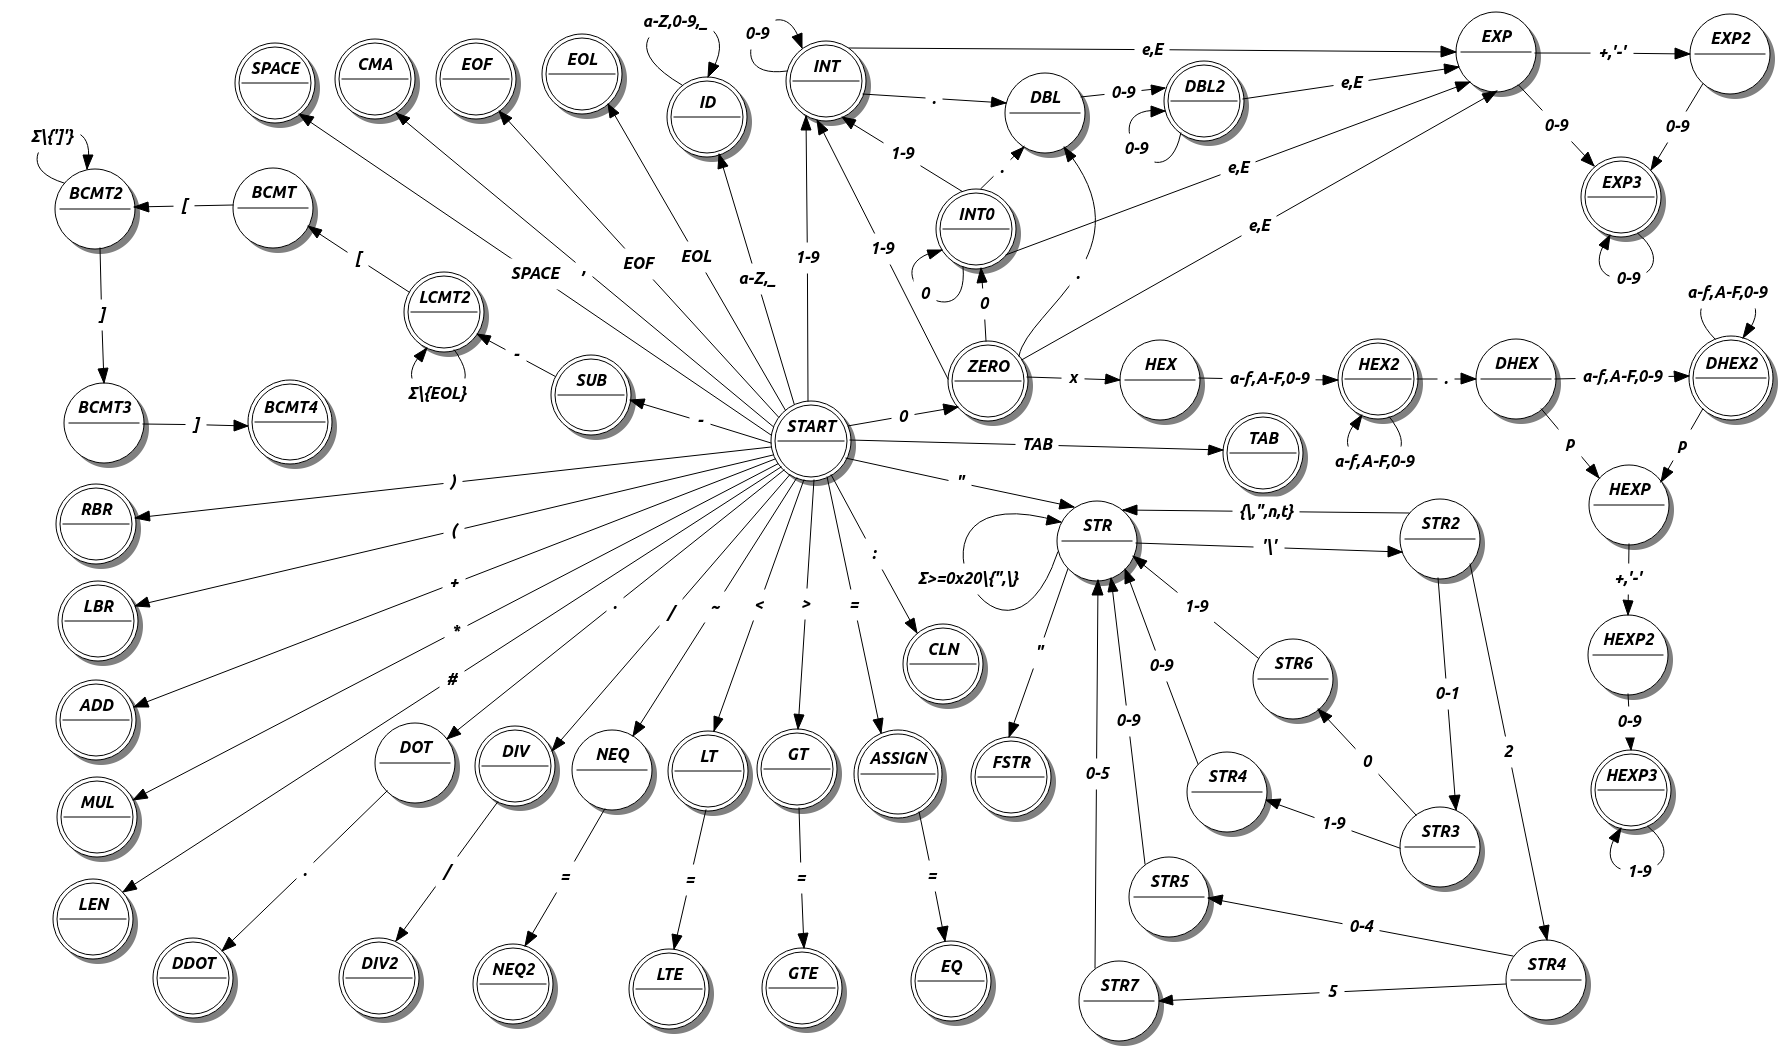
\includegraphics[width=\textwidth,height=\textheight,keepaspectratio]{LexAnalyzatorFSM.png}
    \end{sidewaysfigure}
    \newpage
    
    %%%%%%%%%%%%%%%%%%%%%%% Pravidla LL gramatiky %%%%%%%%%%%%%%%%%%%%%%%%%%%%%%%%
  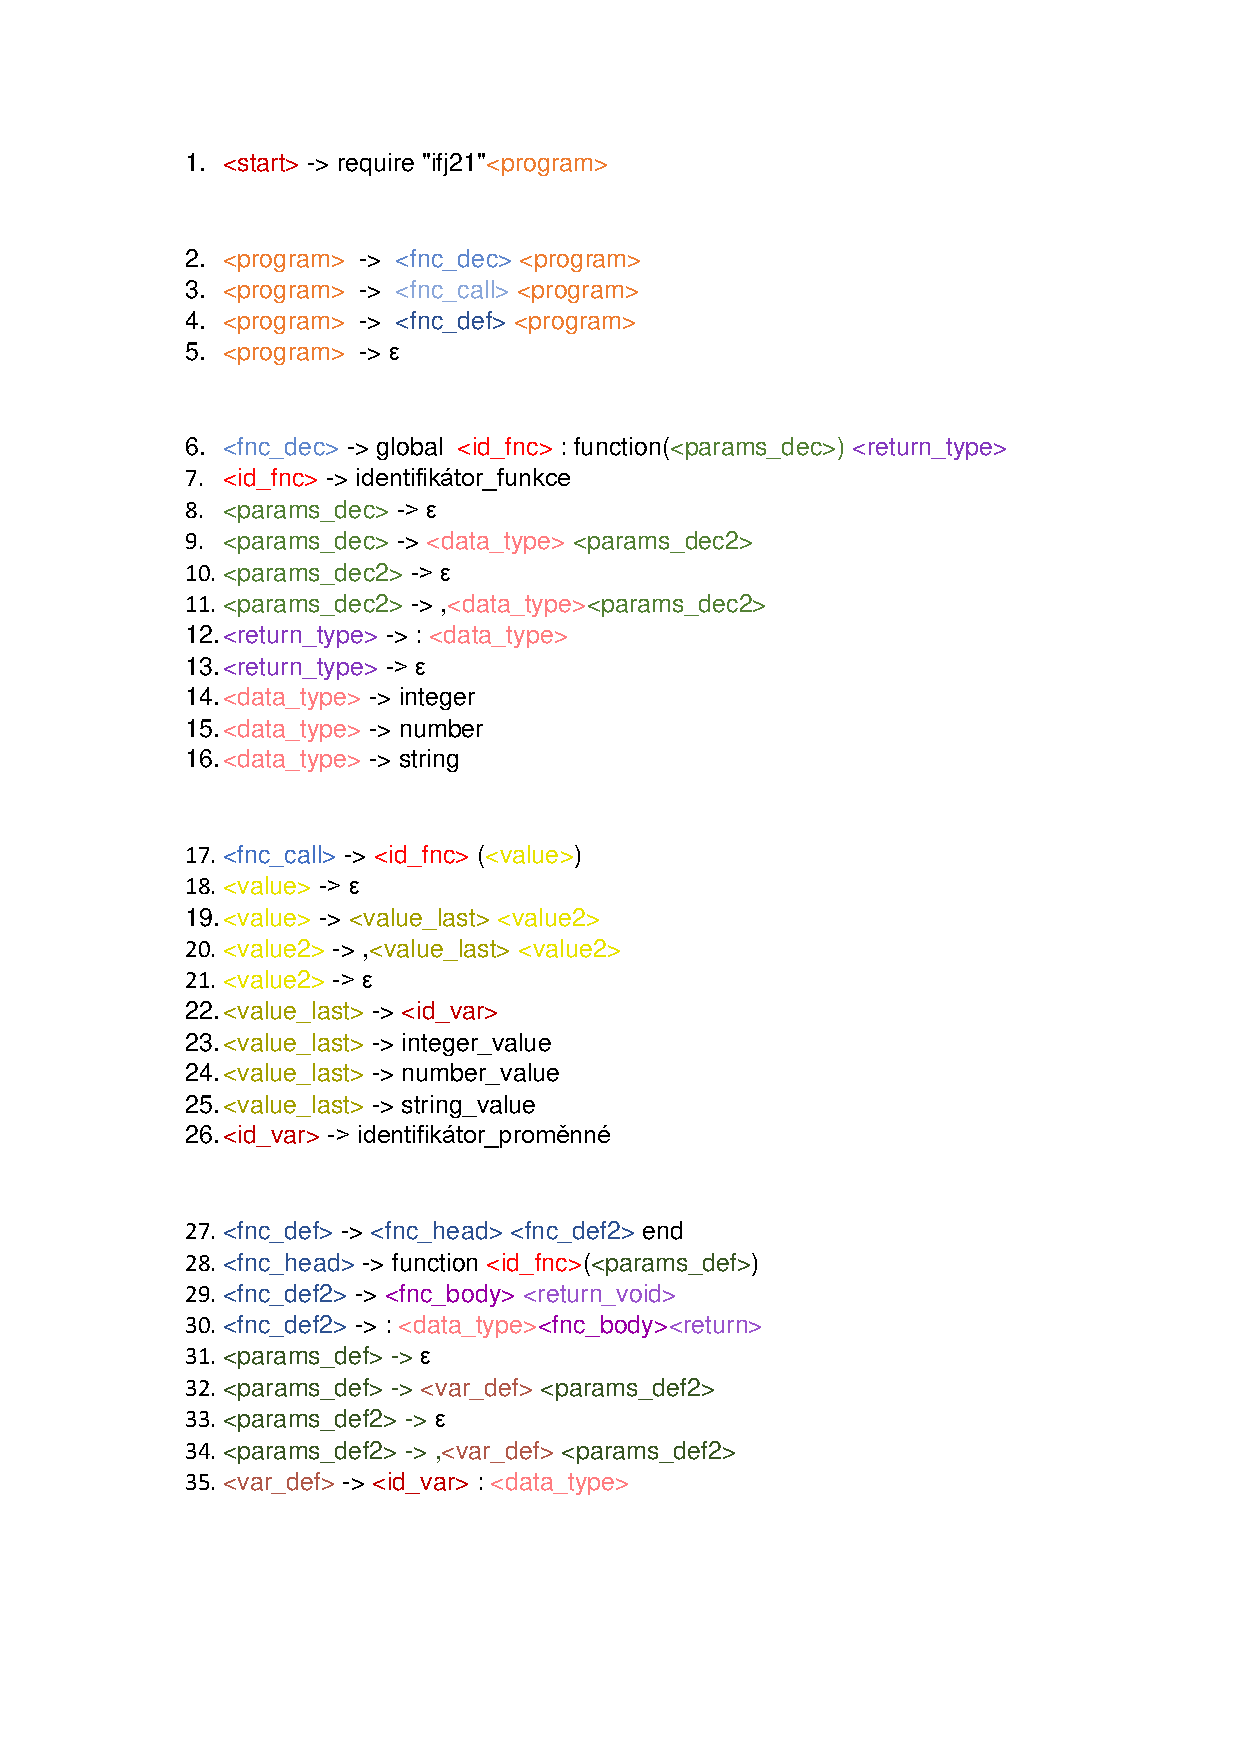
\includepdf[scale=0.83,pages=1,pagecommand=\section{Pravidla LL gramatiky}]{LLGramatika.pdf}
  \includepdf[scale=0.83,pages=2]{LLGramatika.pdf}

	%%%%%%%%%%%%%%%%%%%%%%%%% Precedenční tabulka %%%%%%%%%%%%%%%%%%%%%%%%%%%%%%%%
	\section{Gramatika pro výrazy}
	\begin{enumerate}
 \item EXP $\rightarrow$ i
 \item EXP $\rightarrow$ EXP + EXP
 \item EXP $\rightarrow$ EXP - EXP
 \item EXP $\rightarrow$ EXP * EXP
 \item EXP $\rightarrow$ EXP / EXP
 \item EXP $\rightarrow$ EXP // EXP
 \item EXP $\rightarrow$ EXP .. EXP
 \item EXP $\rightarrow$ (EXP)
 \item EXP $\rightarrow$ EXP $<$ EXP
 \item EXP $\rightarrow$ EXP $>$ EXP
 \item EXP $\rightarrow$ EXP $<$= EXP
 \item EXP $\rightarrow$ EXP $>$= EXP
 \item EXP $\rightarrow$ EXP $\sim$= EXP
 \item EXP $\rightarrow$ EXP == EXP
 \item EXP $\rightarrow$ $\#$EXP
 \end{enumerate}
 \newpage

	%%%%%%%%%%%%%%%%%%%%%%%%% Precedenční tabulka %%%%%%%%%%%%%%%%%%%%%%%%%%%%%%%%
	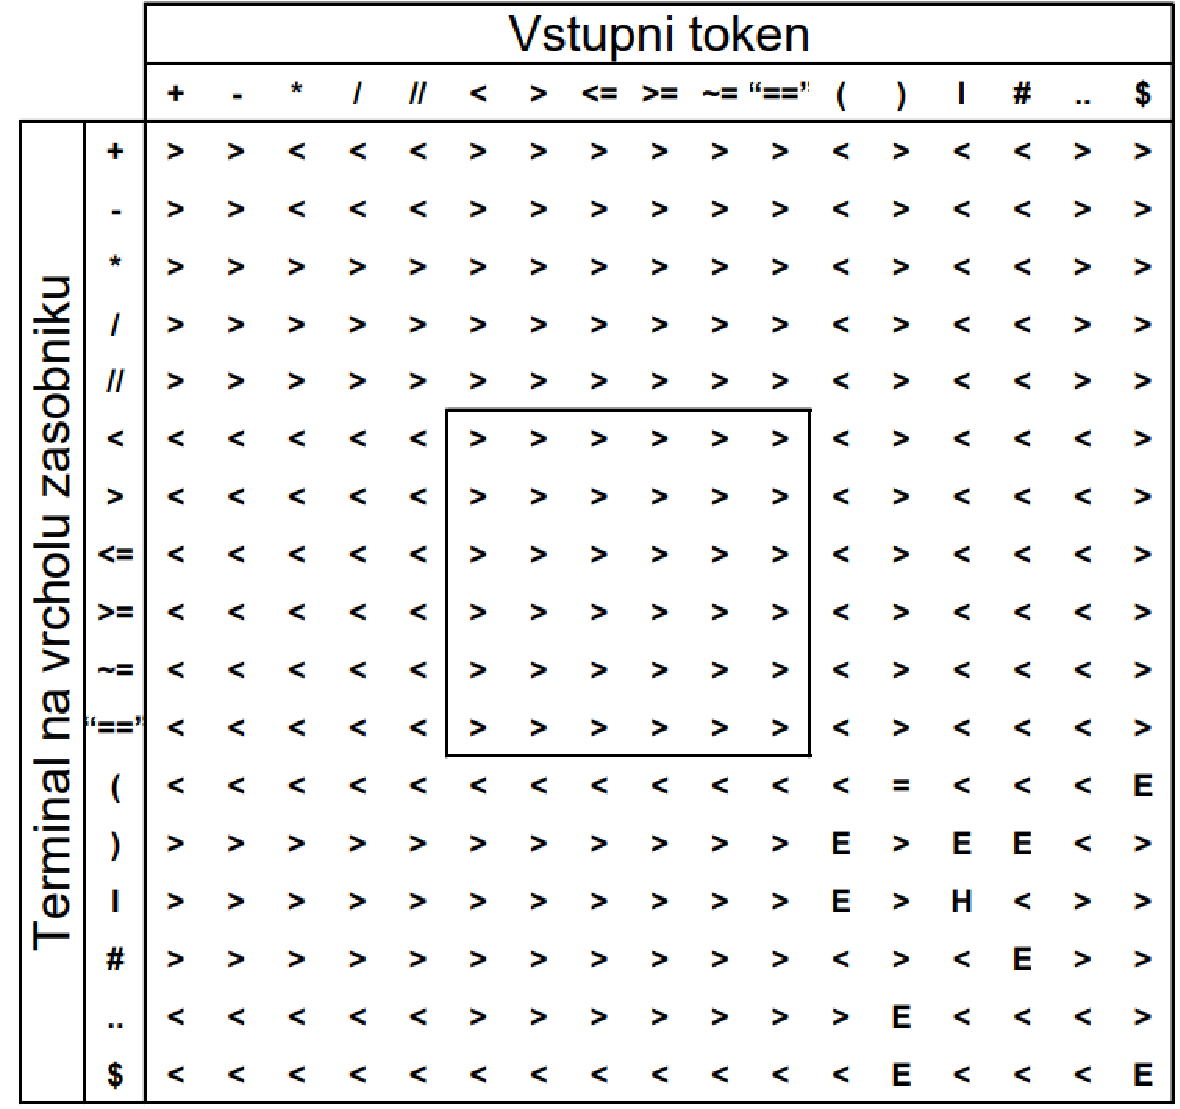
\includepdf[scale=0.83 ,pages=1,pagecommand=\section{Precedenční tabulka}]{precedenceTable.pdf}
 \newpage
 
	%%%%%%%%%%%%%%%%%%%%%%%%%%%%%% Použité zdroje %%%%%%%%%%%%%%%%%%%%%%%%%%%%%%%%
	\section{Použité nástroje, programy a literatura}

\begin{itemize}
\normalsize
  \item Alexandr Meduna a Roman Lukáš, Formální jazyky a překladače, prezentace k přednáškám
  \item Bohuslav Křena, Ivana Burgetová, Algoritmy, prezentace k přednáškám
  \item Zbyněk Křivka, Demonstrační cvičení IFJ, Implementace překladače IFJ21 
  \item Clion, https://www.jetbrains.com/clion/
  \item GitHub, https://github.com/paetricc/IFJ-Project
  \item Vim, https://www.vim.org
  \item QFSM, http://qfsm.sourceforge.net
\end{itemize}

    %%%%%%%%%%%%%%%%%%%%%%%%%%%%%%%% LL tabulka %%%%%%%%%%%%%%%%%%%%%%%%%%%%%%
	\begin{sidewaysfigure}
        \section{LL tabulka}
	        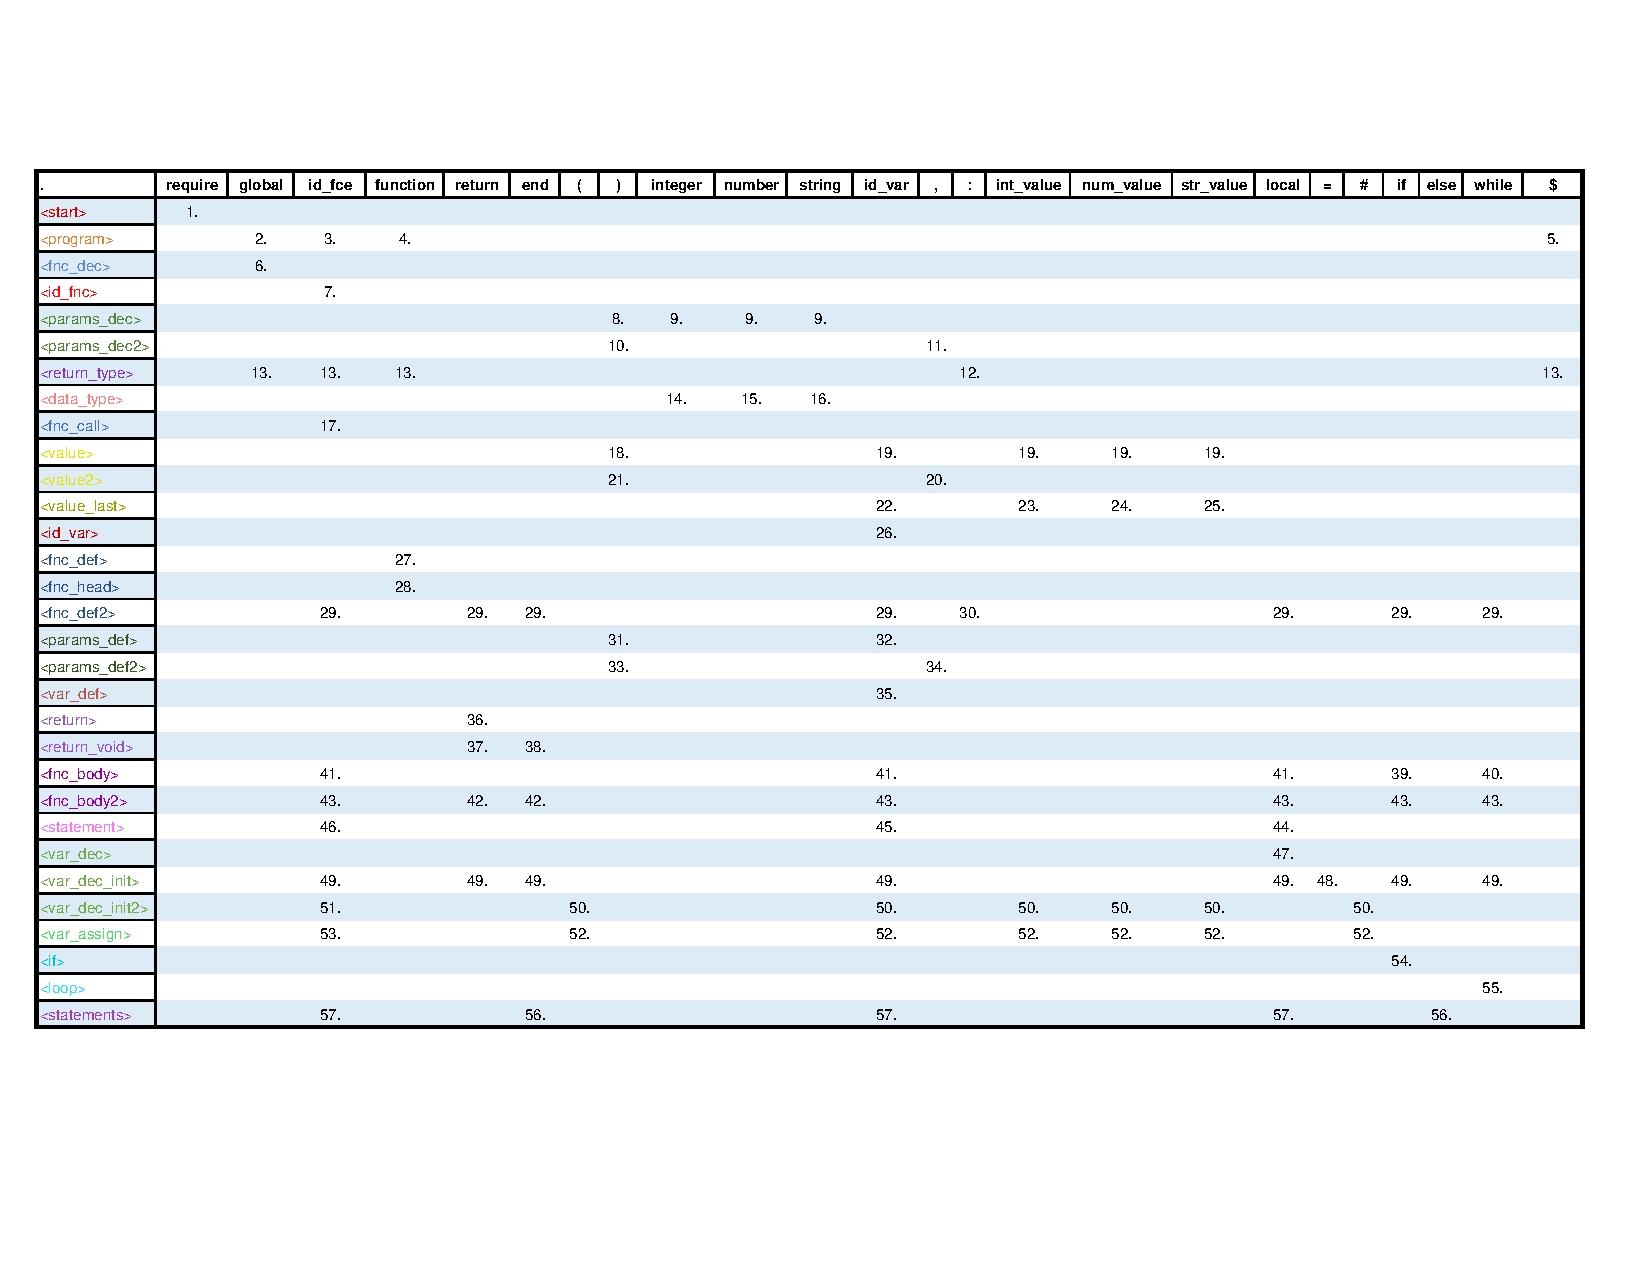
\includegraphics[width=\textwidth,height=\textheight,keepaspectratio]{LLTabulka.pdf}
    \end{sidewaysfigure}
\end{document}